\chapter{Library Evaluation}
\label{cp:eval}

In this Chapter, the library will be evaluated against two simple datasets: MNIST \parencite{lecun1998mnist} and a synthetically generated signal reconstruction dataset. A comparison will be made with equivalent \gls{RVNN} architectures using Tensorflow for the mentioned datasets.  First it will given some brief insights on the performance of this library given its architecture, then some studies regarding adequate learning rates for \gls{CVNN} modulated by the library while being compared with learning rates on \gls{RVNN}. Then training some light \gls{ANN} architectures against these datasets, namely, Multi-Layer Perceptron and a small Convolutional Neural Network. Meanwhile results will be presented alongside a small discussion on each network's performance.

\section{Performance Remarks}
With the development of this library, the focus was not on achieving comparable levels of performance as with \gls{RVNN} frameworks such as Tensorflow. The library was developed without concurrency features, however, it was built with that in mind for adding concurrency if needed. Minimal performance and memory usage optimizations circled around, not cloning data structures and recycling memory as much as possible via references, condensing derivative computations in common loops, and compiling the code with optimization flags.

Having this in consideration for the following results, here are the resultant average runtime of each dataset and architecture per batch:

\begin{table}[h]
	\centering
	\begin{tabular}{llll}
		& FC (22886) & AE (87760) & CNN (32410) \\ \hline
	SR	& - & 531ms & - \\
	MNIST	& 23ms & - & 936ms
	\end{tabular}
	\label{tab:times}
	\caption{Batch run-times in mili-seconds, for the two datasets used (SR stands for the synthetic signal reconstruction dataset) and different architectures with respective number of parameters in parenthesis. FC stands for Fully connected (Multi-Layer Perceptron),  AE is Auto-Encoder, CNN is convolutional neural network.}
\end{table}

\section{\texttt{Renplex}'s Learning Rates}
\label{sec:lr}
To perform the upcoming tests, for each dataset it was performed a series of test with regards to the learning rate. In here, it will be shown for the example of the MNIST dataset using a fully connected architecture showed in Section~\ref{mnist_dense}, how the learning rate was selected. It is noteworthy that the MNIST dataset is not a dataset with complex values, therefore, to feed it to a \gls{CVNN}, one simply defines each pixel as a "complex value" where the imaginary component is null.

To keep the tests short so that the computations would not become to much time expensive, we decided to limit the number of epochs and fit the learning rate so that the model learns in the interval. Fully connected networks learn slower when compared to convolutional neural networks so it was used 32 and 16 epochs respectively.  The criteria used for selecting a learning rate for the referred interval were simple:

\begin{itemize}
	\item Able to stabilize the model for around 5 epochs in the local minimum;
	\item Exhibit little to no oscillations at the local minimum.
\end{itemize}

Figure~\ref{fig:lr_dense_mnist} shows various learning curves with test results (for different learning rates) where values around $ 1.5 $ and $ 2.0 $ appear to be good choices.

\begin{figure}[htbp]
	\centering
	\subfigure[]{
		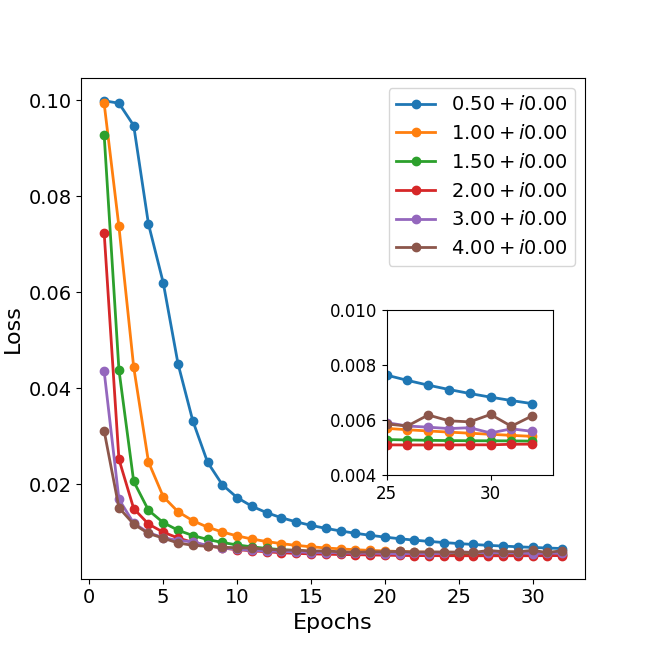
\includegraphics[width=0.45\textwidth]{ch4/assets/lr_dense_mnist_loss.png}
		\label{fig:lr_dense_mnist_loss}
	}
	\subfigure[]{
		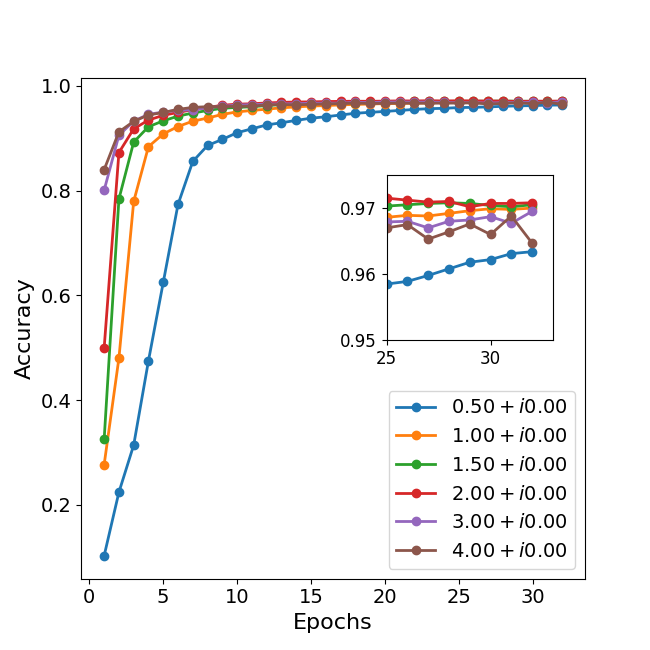
\includegraphics[width=0.45\textwidth]{ch4/assets/lr_dense_mnist_accu.png}
		\label{fig:lr_dense_mnist_accu}
	}
	\caption{Test loss and accuracy curves for the MNIST dataset concerning various real learning rates on the complex-valued multi-layer perceptron for 32 epochs. As the learning rate increases, convergence time improves but also stability decreases.}
	\label{fig:lr_dense_mnist}
\end{figure}

In the study \parencite{zhang2015complex}, shows that it might be beneficial to use an imaginary learning rate to speed up training and achieve slightly results. One of the options is to have a specific adaptive learning rate that can be implemented with the library, however due to its complexity, its implementation was skiped. The other option is to have a small imaginary component, that it is not as beneficial as the adaptive approach but also showed some improvements. The latter was tested and Figure~\ref{fig:lr_im_dense_mnist} shows the results where one can see that there is this slight benefit in convergence time but, for this case, the local minimum value is around the same for each curve.

\begin{figure}[htbp]
	\centering
	\subfigure[]{
		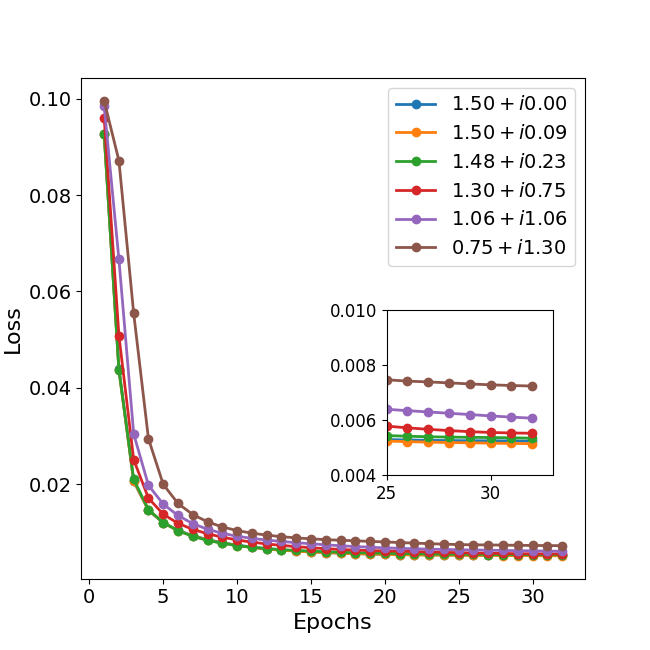
\includegraphics[width=0.45\textwidth]{ch4/assets/lr_im_dense_mnist_loss.png}
		\label{fig:lr_im_dense_mnist_loss}
	}
	\subfigure[]{
		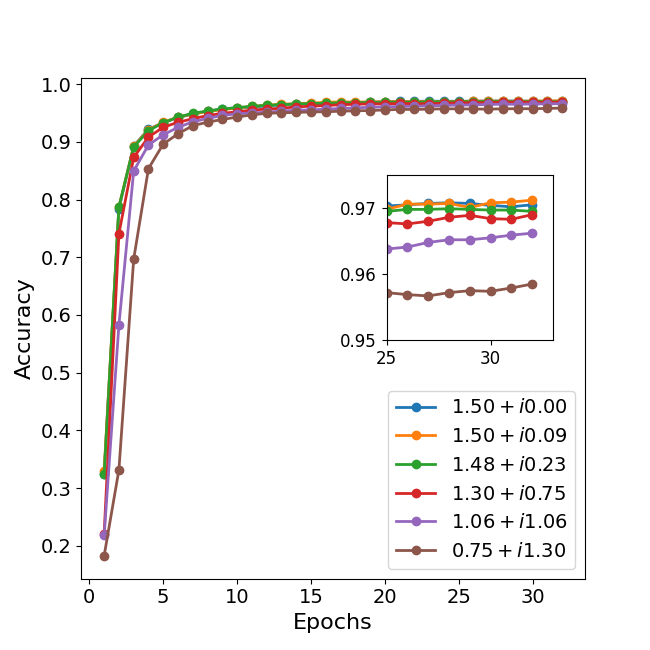
\includegraphics[width=0.45\textwidth]{ch4/assets/lr_im_dense_mnist_accu.png}
		\label{fig:lr_im_dense_mnist_accu}
	}
	\caption{Test loss and accuracy curves for the MNIST dataset concerning various imaginary learning rates on the complex-valued multi-layer perceptron for 32 epochs. The studied learning rates follow an increase in phase with values $ 0 $, $ \frac{\pi}{20} $, $ \frac{\pi}{10} $, $ \frac{\pi}{6} $, $ \frac{\pi}{4} $ and $ \frac{\pi}{3} $ with absolute value of $ 1.50 $.}
	\label{fig:lr_im_dense_mnist}
\end{figure}

The process discussed just now, was also applied for every Tensorflow architecture developed. In the same context, Figure~\ref{fig:lr_dense_mnist_tf} shows learning curves obtained with equivalent architecture with Tensorflow. One can notice that, such  learning rates are slightly higher and learning curves more unstable when compared with the CVNN architecture, in other words, Tensorflow, has more difficulty training the model in the same amount of epochs that the CVNN does with stability (and higher accuracy).

\begin{figure}[htbp]
	\centering
	\subfigure[]{
		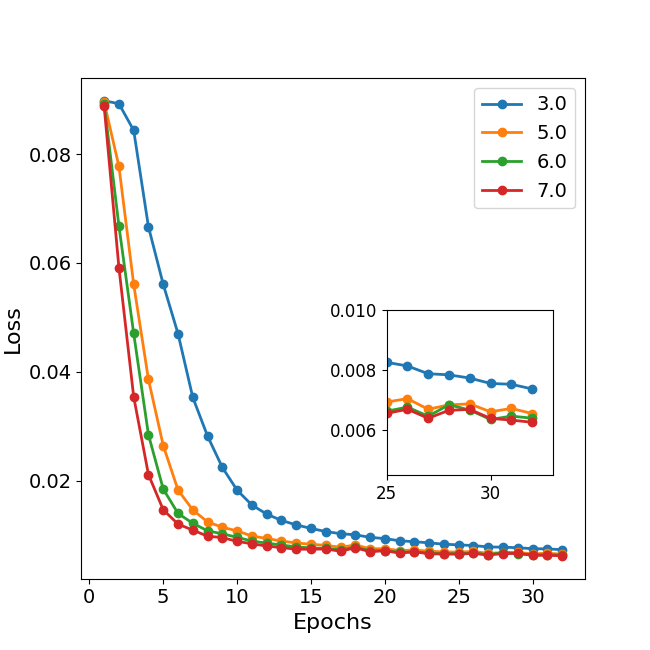
\includegraphics[width=0.45\textwidth]{ch4/assets/lr_dense_mnist_loss_tf.png}
		\label{fig:lr_dense_mnist_loss_tf}
	}
	\subfigure[]{
		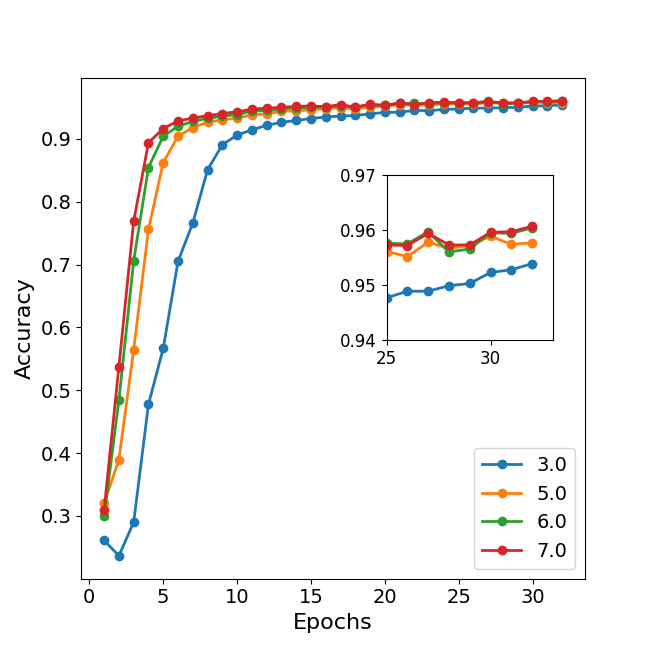
\includegraphics[width=0.45\textwidth]{ch4/assets/lr_dense_mnist_accu_tf.png}
		\label{fig:lr_dense_mnist_accu_tf}
	}
	\caption{Test loss and accuracy curves using Tensorflow for the MNIST dataset concerning various learning rates on the multi-layer perceptron for 32 epochs.}
	\label{fig:lr_dense_mnist_tf}
\end{figure}

\section{Fully Connected Neural Network Applications}
The current section will show two distinct applications of fully connected CVNN. First, a layout for classification using the MNIST dataset, then an auto-encoder type of architecture using dense layers for signal reconstruction. For the purpose of proving that the library works as intended, while minimizing runtime, the focus will be on very simple architectures constructed for the purpose of this Master Thesis only.

On a side note, it is important to note that, since the implementation of cross entropy Loss function is not well defined or explored in the literature, we used the mean squared error loss function for both Renplex and Tensorflow. This is without loss of generality since the derivative of the cross entropy (in composition with the softmax activation that is necessary), is the same as the derivative of the mean squared error, so the derivatives are propagated equally in both scenarios. This only plays a roll in optimization algorithms that pick up the loss function values for determining next iterations of the learning rate, which is also something that we will not be addressing in this simple case of studies.

\subsection{MNIST Dataset}
\label{mnist_dense}

The task at hand with this dataset is: given a single channel input image of $ 28 \times 28 $ pixels containing a handwritten digit, train the network to identify which digit is. For such, that output layer will need have 10 units where the neuron with greatest activation classifies the digit it represents. Based on the Multi-Layer Perceptron architecture \parencite{rumelhart1986}, we will suggest for this study the following architecture consisting of 5 layers in total:

\begin{itemize}
	\item 1 - Flatten Layer to map the $ 28 \times 28 $ matrix to a vector of dimension $ 784 $;
	\item 2 - Dense Layer, 28 units, (split) sigmoid activation;
	\item 3 - Dense Layer, 16 units, (split) sigmoid activation;
	\item 4 - Dense Layer, 16 units, (split) sigmoid activation;
	\item 5 - Dense Layer, 10 units, (split) sigmoid activation.
\end{itemize}

The differences between RVNN and CVNN architectures are marked with the parenthesis. Instead of having the sigmoid activation function, one has an equivalent one which we choose to be and Real-Imaginary-Type or split sigmoid function,

\begin{equation}
	\sigma_{S}(z) = \sigma\group{\Real{z}} + i\sigma\group{\Imag{z}}.
\end{equation}

With this setup the following results in Figure~\ref{fig:comp_dense_mnist} were obtained. These results, as the followings, were obtained by running 6 different random seeds through 32 epochs and averaging out all points of all learning curves obtained, then drawing the mean learning curve inside a region with the size of plus/minus 2 times the standard deviation of each epoch value. For both networks, it was used batches of $ 100 $ images and the default data split with the MNIST dataset (the same for all instances where we study MNIST in this master thesis).

\begin{figure}[htbp]
	\centering
	\subfigure[]{
		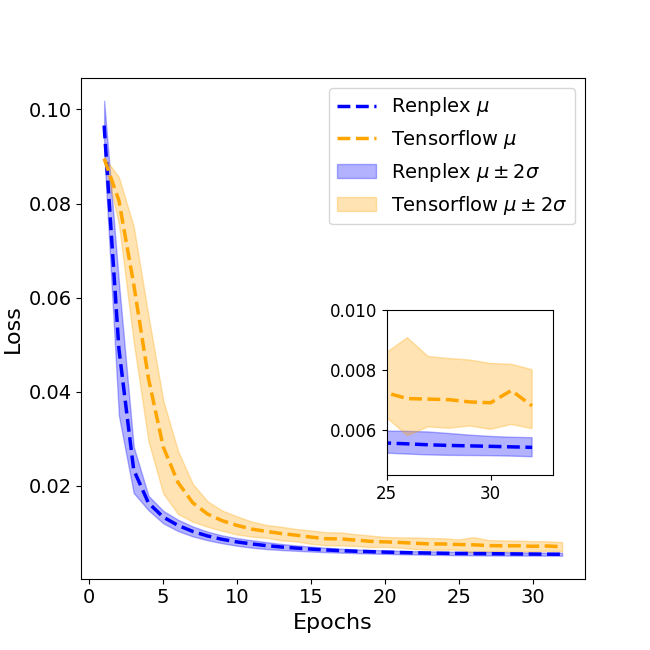
\includegraphics[width=0.45\textwidth]{ch4/assets/comp_dense_mnist_loss.png}
		\label{fig:comp_dense_mnist_loss}
	}
	\subfigure[]{
		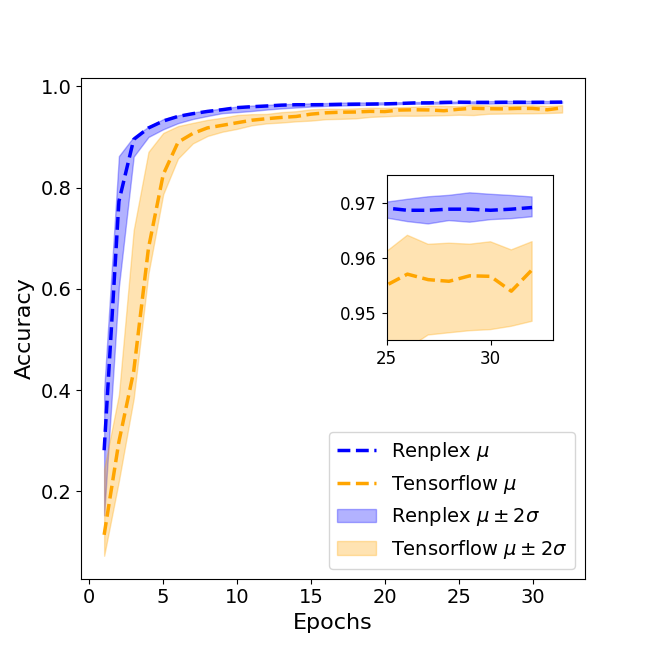
\includegraphics[width=0.45\textwidth]{ch4/assets/comp_dense_mnist_accu.png}
		\label{fig:comp_dense_mnist_accu}
	}
	\caption{Comparison of mean test loss and accuracy curves between Renplex and Tensorflow for the MNIST dataset with equivalent multi-layered perceptron-based neural network models. The $ \mu $ represents the average curve of all learning curves concerning 6 seeds, and $ 2\sigma $ two times the standard deviation related to every loss and accuracy value for each of the $ 32 $ epochs.}
	\label{fig:comp_dense_mnist}
\end{figure}

The results show that the \gls{CVNN} over-performed the \gls{RVNN} and even offered greater stability when reaching the local minimum. Additionally, CVNN seemed to have converged in less epochs compared to the RVNN. We would also like to note that the selected learning rates were in accordance with the pipeline in Section~\ref{sec:lr}, as will all the results in this chapter.

\subsection{Synthetic Signal Reconstruction Dataset}
In this next test of the library,the task that was performed was discussed in the state-of-the-art as very common to be executed by a \gls{CVNN}. The network will be provided a noisy (complex) signal and its objective is to guess what the clean signal $ s(t) $ is behind the noise. For this task we generated a Synthetic Dataset.

\subsubsection{Method for Generating the Dataset}
To generate this dataset we first considered a plain wave signal,

\begin{equation}
	y(t) = \rho e^{i(\omega t + \phi)}
\end{equation}
where $ \rho $ is the amplitude, $ \omega $ frequency and $ \phi $ the phase of the signal. In a more practical sense, $ t $ is the sampling vector or simply the time variable.

One way one could generate the dataset is by generating a various random combinations of $ \rho $, $ \omega $ and $ \phi $, produce a signal $ y_i(t) $, which would be the dependent variable, and then add Gaussian noise to it to get $ x_i(t) $ being each respective independent variable. Nevertheless, for this dataset we decided to form more complex (normalized) signals composed of multiple plain waves like so,

\begin{equation}
	y(t) = C \sum_n^{N} \rho_n e^{i(\omega_n t + \phi_n)},
\end{equation}
where $ C $ is some normalization constant, the amplitudes and frequencies $ \rho_n $ and $ \omega_n $ respectively, were both randomly uniformly distributed between $ 0.1 $ and $ 1 $ and all $ \phi_n $ were uniformly distributed between $ 0 $ and $ 2\pi $. The number of waves $ N $, for each signal $ y(t) $ of the dataset, were integers randomly uniformly distributed between $ 1 $ and a given limit number of waves to add which we considered $ 8 $ for upcoming tests. To have on average at least one complete cycle of the signal, the vector $  t $ goes from $ 0 $ to $ 4\pi $ with $ 512 $ samples.

To generate the dependent variables, i.e. noisy input signal to the network $ x(t) $, one would just add Gaussian noise $ g_\sigma(t) $ with a mean of $ 0 $ and a defined standard deviation governed by a threshold $ \sigma_0 $ which in the following cases was $ 0.025 $. To have a proportional noise to intensity, the former was used and a threshold for noise and increased with the sample's intensity by the following expression,

\begin{equation}
	\sigma = \sigma_0 \group{1 + \dfrac{\norm{y(t)}}{20}},
\end{equation}
for every given instant $ t $ such that $ x(t) = y(t) + g_\sigma(t) $. On Figure~\ref{fig:sig_dataset} we show four examples of pairs $ (x(t), y(t)) $ used for the dataset were one can see that multiple amplitudes and frequencies might be contained on the signal and that the noise remains proportional throughout different absolute values of the samples.

\begin{figure}[htbp]
	\centering
	\subfigure[]{
		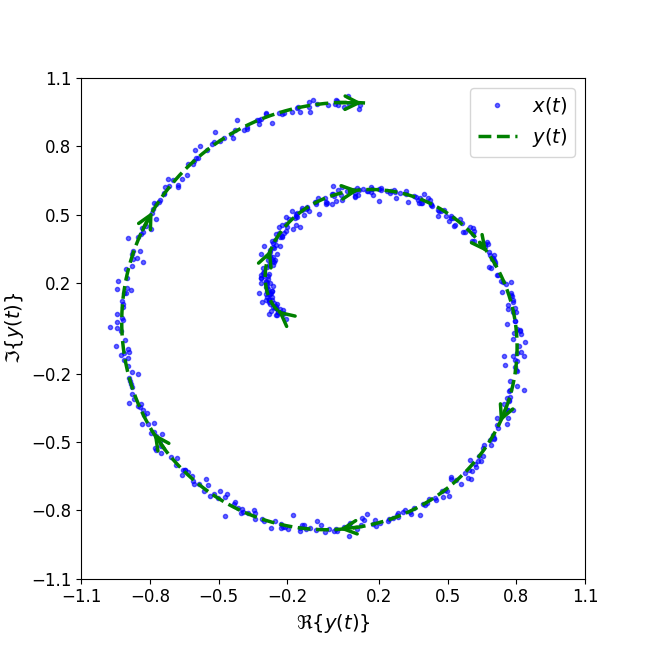
\includegraphics[width=0.45\textwidth]{ch4/assets/sig1_dataset.png}
		\label{fig:sig1_dataset}
	}
	\subfigure[]{
		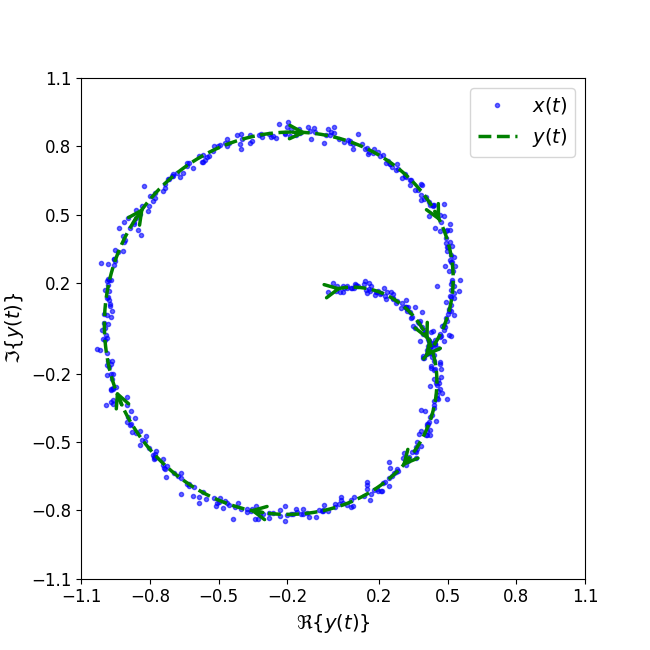
\includegraphics[width=0.45\textwidth]{ch4/assets/sig2_dataset.png}
		\label{fig:sig2_dataset}
	}
	\subfigure[]{
		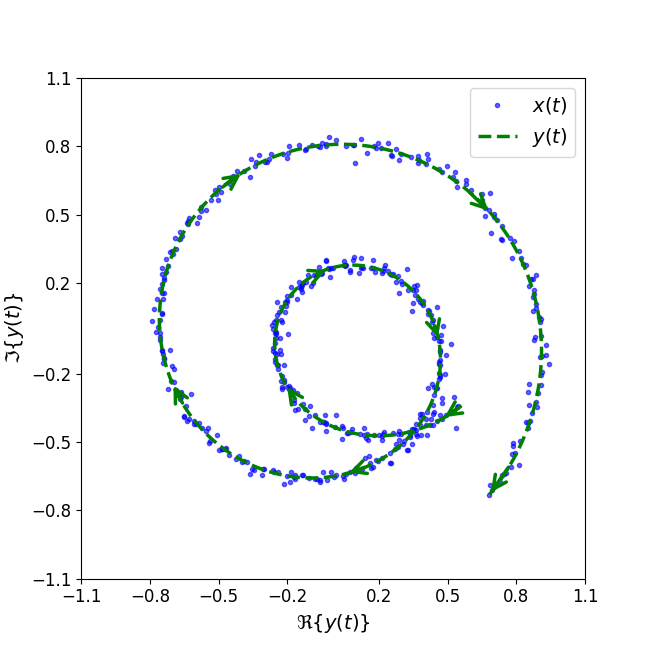
\includegraphics[width=0.45\textwidth]{ch4/assets/sig3_dataset.png}
		\label{fig:sig3_dataset}
	}
	\subfigure[]{
		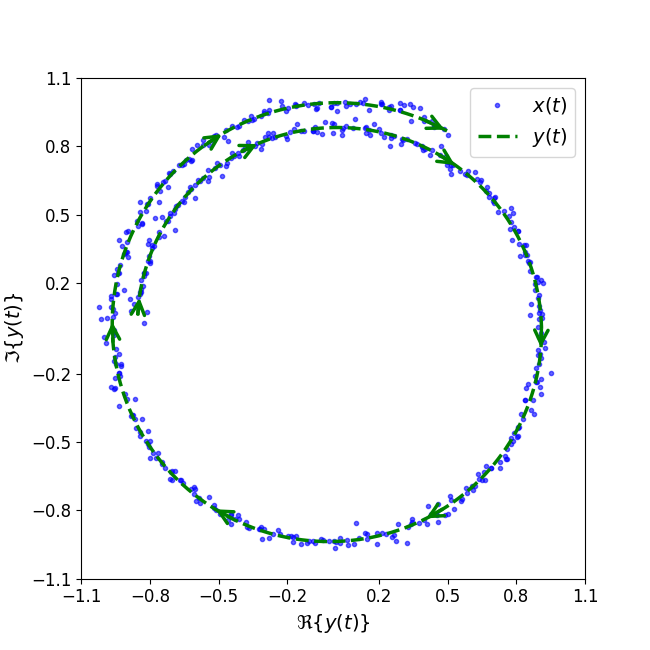
\includegraphics[width=0.45\textwidth]{ch4/assets/sig4_dataset.png}
		\label{fig:sig4_dataset}
	}
	\caption{Four pairs of independent $ x(t) $ and dependent variables $ y(t) $ from the signal reconstruction dataset. Samples are represented in the complex plane, in green the supposed smooth signal and in blue dots the signal with Gaussian Blur. Arrows indicate the direction of propagation of the signal.}
	\label{fig:sig_dataset}
\end{figure}

Regarding training and testing data, $ 20000 $ pairs of noisy and clean signal respectively were generated for both training and testing pipeline. All formed with random number of waves each with its own unique and random amplitudes, frequencies and phases.

\subsubsection{Results}
To extract the results in Figure~\ref{fig:comp_dense_sig_loss}, it was used the \gls{CVNN} architecture equivalent to the Auto-Encoder one. It consisted of:

\begin{itemize}
	\item 1 - Dense Layer, 128 units, (split) hyperbolic tangent activation. (This layer receives the signal encoded in a vector with 512 elements);
	\item 2 - Dense Layer, 32 units, (split) hyperbolic tangent activation;
	\item 3 - Dense Layer, 16 units, (split) hyperbolic tangent activation;
	\item 4 - Dense Layer, 32 units, (split) hyperbolic tangent activation;
	\item 5 - Dense Layer, 512 units, no activation.
\end{itemize}

However, since the signal is complex in its nature, one needs to find a way to feed it to a \gls{RVNN}. In Tensorflow, it was created two equal networks where one trains on the real part of the signal and the other on the imaginary part of the signal. The predicted outputs of each model are combined in a single output and loss is then calculated according to the error in equation (\ref{eq:error_cp}). This studies in Figure~\ref{fig:comp_dense_sig_loss} were performed for 32 epochs and to select the learning rate an additional note was taken into account: output signals must have little to no signal-to-noise-ratio. If a small enough learning rate is given in such a task, the network simply tries to minimize the mean squared loss with no consideration whatsoever to the noise of the prediction, yielding at the end a very good result in terms of loss, but something that does not resembles a clear signal. 

\begin{figure}[htbp]
	\centering
	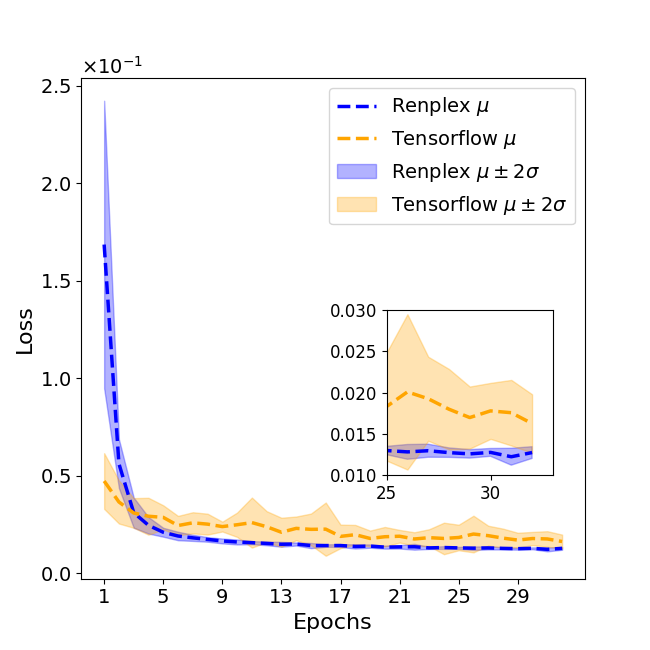
\includegraphics[width=0.45\textwidth]{ch4/assets/comp_dense_sigrec_loss.png}
	\caption{Comparison of mean test loss and accuracy curves between Renplex and Tensorflow for the Synthetic Signal Reconstruction dataset with equivalent auto-encoder-based neural network models. The $ \mu $ represents the average curve of all learning curves concerning 6 seeds, and $ 2\sigma $ two times the standard deviation related to every loss and accuracy value for each of the $ 32 $ epochs.}
	\label{fig:comp_dense_sig_loss}
\end{figure}

These results show again that a CVNN model outperforms RVNN model and also offer more stability while converging to a local minimum, in spite of initiating training at slightly worst loss values. Additionally it also trains quicker epoch-wise since it soon over-took the RVNN more or less at the 4 epoch mark. The capability of generalization becomes apparent if we visualize some predictions made from both CVNN and RVNN in Figure~\ref{fig:signals}. This figure suggests that, a RVNN has difficulties in continuously curving the signal in the complex plane, executing less smooth curves when compared to a CVNN prediction. Another disadvantage of the RVNN model is that it was used a "split-model" where one creates two independent models, one to deal with the real part and another to deal with the imaginary part of the signal, which is double the memory. The other option for the RVNN would be to have an input of 1024 (far all real and imaginary values separately) instead of 512 but that would be changing the architecture to much. Additionally, it actually produced less accurate results when compared to the split model.

\begin{sidewaysfigure}
	\centering
	\begin{minipage}{\linewidth}
		\centering
		\subfigure[]{
			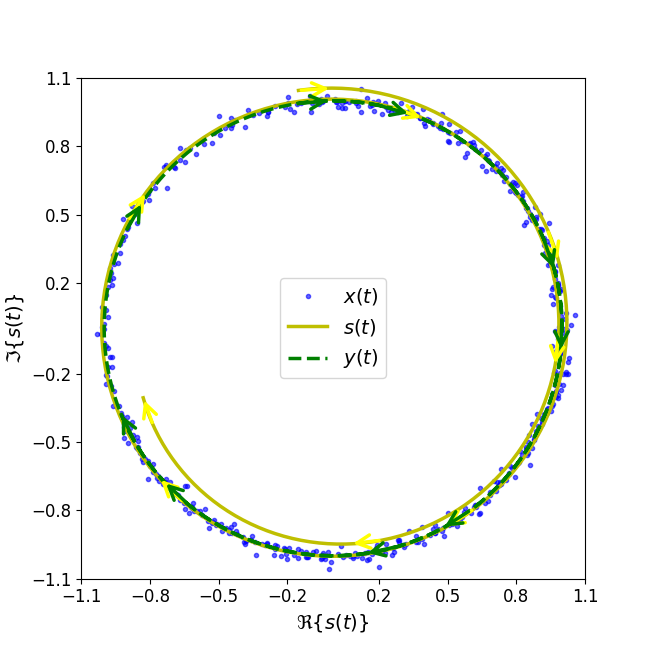
\includegraphics[width=0.2\textwidth]{ch4/assets/re_sin.png}
			\label{fig:ren_sig0}
		}
		\subfigure[]{
			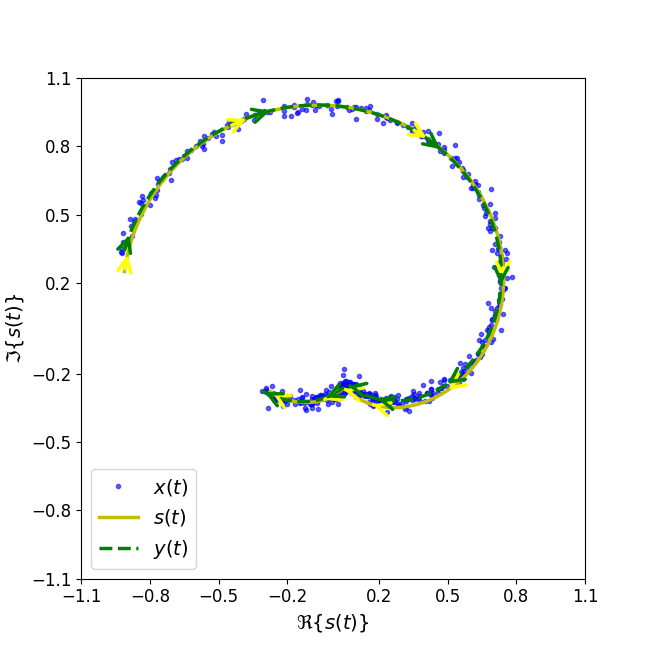
\includegraphics[width=0.2\textwidth]{ch4/assets/re_wow.png}
			\label{fig:ren_sig1}
		}
		\subfigure[]{
			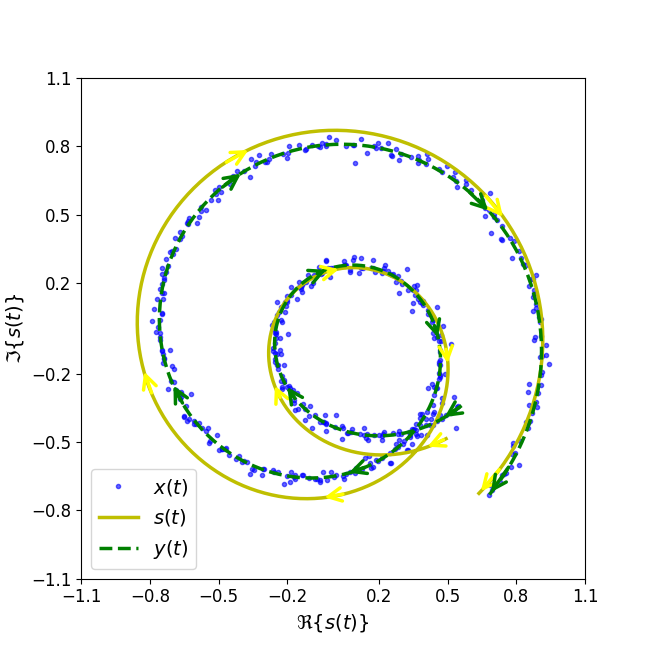
\includegraphics[width=0.2\textwidth]{ch4/assets/re_mega_schneke.png}
			\label{fig:ren_sig2}
		}
		\subfigure[]{
			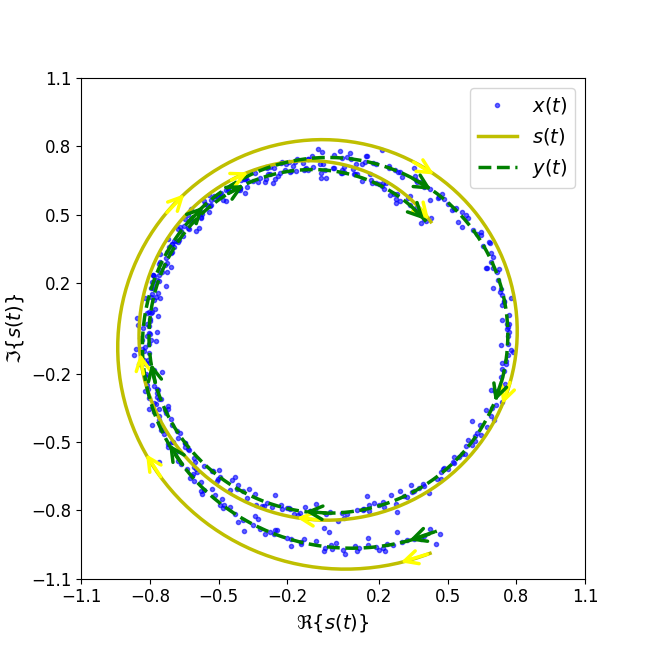
\includegraphics[width=0.2\textwidth]{ch4/assets/re_almost_sin.png}
			\label{fig:ren_sig3}
		}
	\end{minipage}

	\begin{minipage}{\linewidth}
		\centering
		\subfigure[]{
			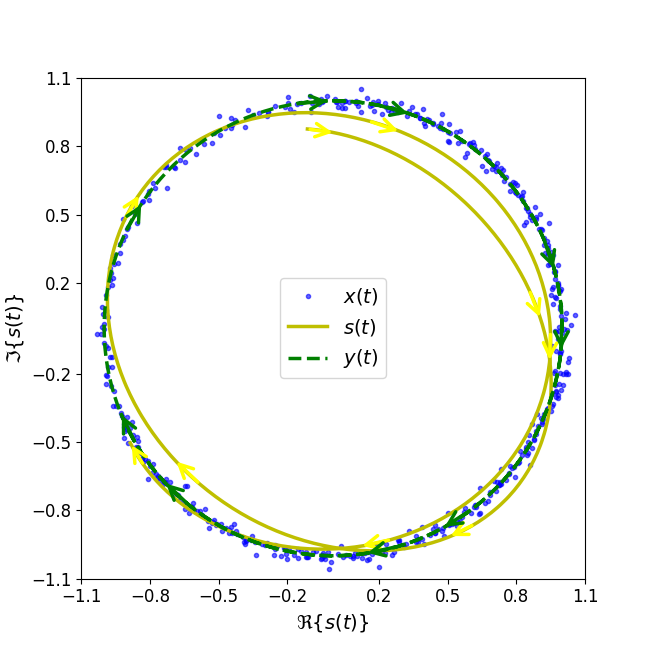
\includegraphics[width=0.2\textwidth]{ch4/assets/tf_sin1.png}
			\label{fig:tf_sig0}
		}
		\subfigure[]{
			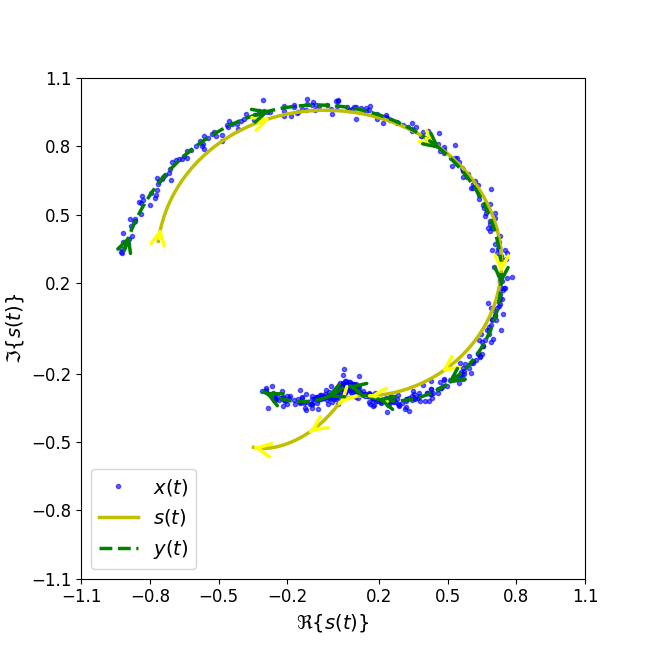
\includegraphics[width=0.2\textwidth]{ch4/assets/tf_notwow.png}
			\label{fig:tf_sig1}
		}
		\subfigure[]{
			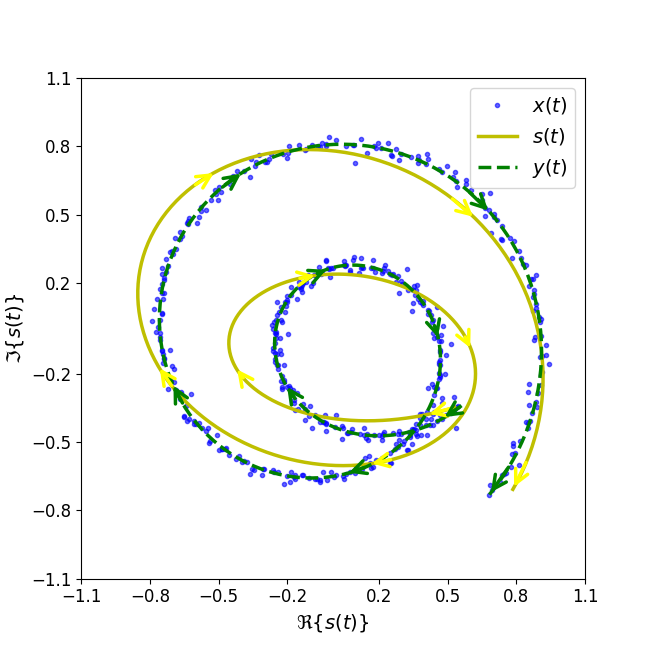
\includegraphics[width=0.2\textwidth]{ch4/assets/tf_stupid_schneke.png}
			\label{fig:tf_sig2}
		}
		\subfigure[]{
			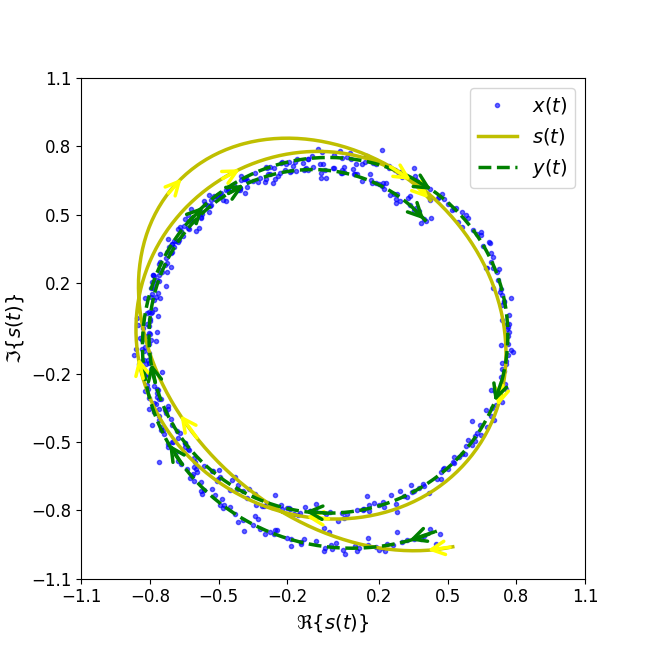
\includegraphics[width=0.2\textwidth]{ch4/assets/tf_almost_sin.png}
			\label{fig:tf_sig3}
		}
	\end{minipage}
	\caption{A set of 4 predictions in yellow ($ s(t) $) executed from by the Renplex model from (a) to (d) and Tensorflow model(s) from (e) to (h). Tensorflow here is using two models in parallel, one for dealing with the real and the other for the imaginary part. $ x(t) $ is the Gaussion noise version of $ y(t) $ and $ s(t) $ the attempt for reconstruction of $ y(t) $. Signals in (a) and (e) are pure plane waves and the rest contain multiple frequencies (up to 8).}
	\label{fig:signals}
\end{sidewaysfigure}

\section{Convolutional Neural Network Applications}
Since the library is also capable of performing 2D convolutions, this section shows a simple application of a \gls{CVNN} in comparison with a \gls{RVNN}, in the same classification task with the MNIST dataset. This example will consist in a light Convolutional Neural Network architecture where the convolutional operation inside the complex convolution layer is performed according to what was described in Section~\ref{sec:2Dconv}.

\subsection{MNIST Dataset}
It was decided to use the MNIST dataset and an architecture that did not involved a considerable amount of parameters. It consisted in:
 
 \begin{itemize}
 	\item 1 - Convolutional Layer, $  8 $ filters, $ 3 \times 3 $ kernel size, (split) ReLU activation;
 	\item 2 - Average Pooling Layer (showed in Section~\ref{lst:avg_pool}), $ 2 \times 2 $ block;
 	\item 3 - Convolutional Layer, $ 16 $ filters, $ 3 \times 3 $ kernel size, (split) ReLU activation;
 	\item 4 - Dense Layer, $ 16 $ units, (split) sigmoid activation;
 	\item 5 - Dense Layer, $ 10 $ units, (split) sigmoid activation.
 \end{itemize}
 
The $ 8 $ input filters, make sure that first layer's activation does not store a lot of features, substantially reducing memory usage, and to make sure that the convolution layer performs the major role on the task, a reduced number of Dense units was added. Tests ran for $ 16 $ epochs due to these types of networks training faster but also more time expensive. Result on Figure~\ref{fig:comp_cnn_mnist}, show a comparable performance between the RVNN and CVNN both in accuracy and solution stability.

In spite of the network modeling being almost analogous between RVNN and CVNN, it is important to notice that Tensorflow does not incorporate fractional up-sampling as a method for propagating derivatives backwards through the average polling layer. In fact, it has a method much more reliable almost mimicking the inverse process of the average pooling \parencite{tensorflow2023}. In Renplex's case, for easiness in implementation and quick release of the library, we decided to have a common operation for propagating derivatives through the Reduce Layer which is not ideal and may hinder performance.

\begin{figure}[htbp]
	\centering
	\subfigure[]{
		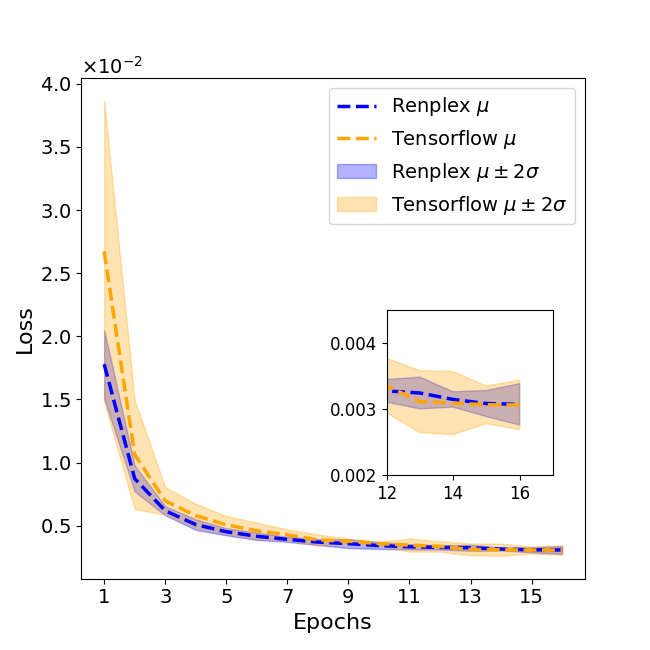
\includegraphics[width=0.45\textwidth]{ch4/assets/comp_cnn_mnist_loss.png}
		\label{fig:comp_cnn_mnist_loss}
	}
	\subfigure[]{
		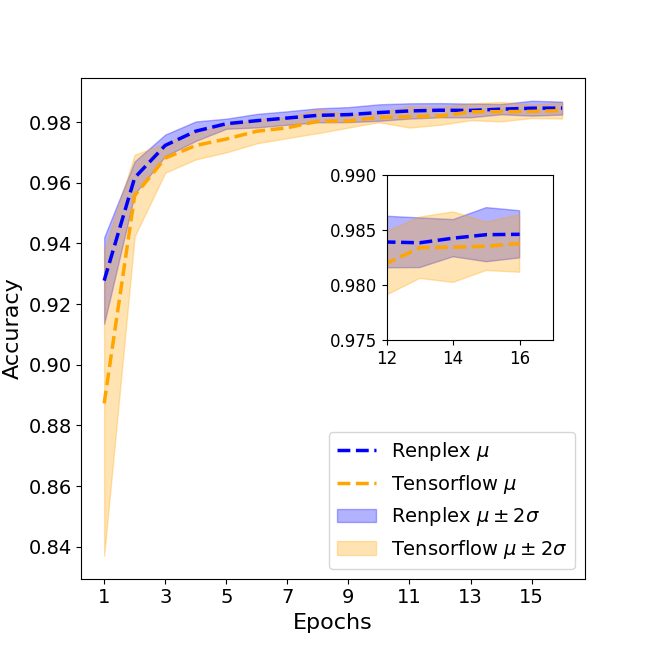
\includegraphics[width=0.45\textwidth]{ch4/assets/comp_cnn_mnist_accu.png}
		\label{fig:comp_cnn_mnist_accu}
	}
	\caption{Comparison of mean test loss and accuracy curves between Renplex and Tensorflow for the MNIST dataset with equivalent convolutional-based neural network models. The $ \mu $ represents the average curve of all learning curves concerning 6 seeds, and $ 2\sigma $ two times the standard deviation related to every loss and accuracy value for each epoch.}
	\label{fig:comp_cnn_mnist}
\end{figure}

When the process of training these models was finished, we extracted the output feature maps from the first convolutional layer (input layer) and collected them in Figures \ref{fig:feats},  \ref{fig:featscxy} and \ref{fig:featsc}. In the first, we show output feature maps from the RVNN modeled by Tensorflow where one can see some high-level features like image smoothing, contrasts and edge detection. In the second and third results, we show the complex output features maps from two different perspectives in the same CVNN. 

It might be confusing to see MNIST images colored, however, since inside the CVNN features have complex-valued pixels, we decided to map on Figure~\ref{fig:featscxy}, the real part of the pixel to shades of red and the imaginary part in shades of green. In Figure~\ref{fig:featscxy}, the absolute values of the pixel are mapped to shades of red and their phases in shades of green. One can see from these results, that from both perspectives, the CVNN tried to capture some high-level features and transitions. Sometimes bringing the input image completely to the imaginary axis, or sometimes encoding sections of the input image with different phase values.

\begin{sidewaysfigure}
	\centering
	\subfigure[]{
		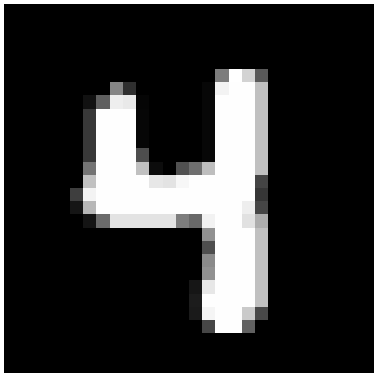
\includegraphics[width=\sideimagewidth]{ch4/assets/4_tf_original.png}
		\label{fig:feat_ori}
	}
	\subfigure[]{
		
\includegraphics[width=\sideimagewidth]{ch4/assets/4_tf_feat0.png}
		\label{fig:feat0}
	}
	\subfigure[]{
		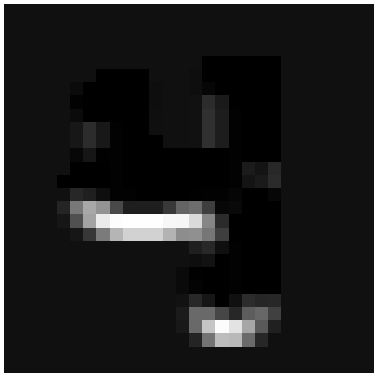
\includegraphics[width=\sideimagewidth]{ch4/assets/4_tf_feat1.png}
		\label{fig:feat1}
	}
	\subfigure[]{
		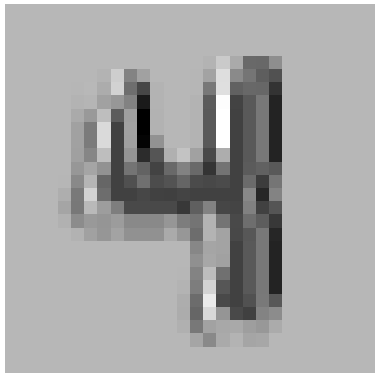
\includegraphics[width=\sideimagewidth]{ch4/assets/4_tf_feat2.png}
		\label{fig:feat2}
	}
	\subfigure[]{
		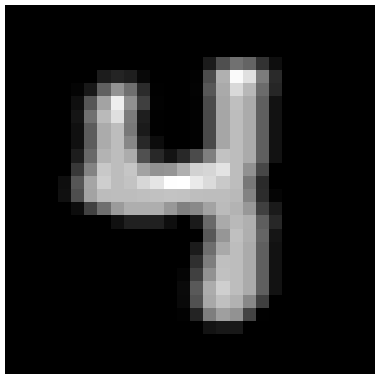
\includegraphics[width=\sideimagewidth]{ch4/assets/4_tf_feat3.png}
		\label{fig:feat3}
	}
	\subfigure[]{
		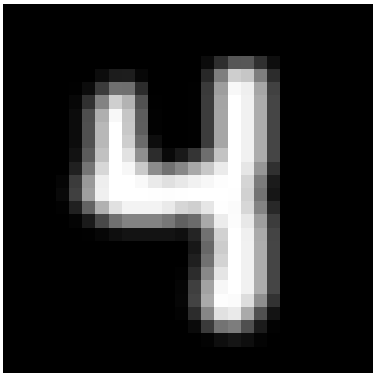
\includegraphics[width=\sideimagewidth]{ch4/assets/4_tf_feat4.png}
		\label{fig:feat4}
	}
	\subfigure[]{
		
\includegraphics[width=\sideimagewidth]{ch4/assets/4_tf_feat5.png}
		\label{fig:feat5}
	}
	\subfigure[]{
		
\includegraphics[width=\sideimagewidth]{ch4/assets/4_tf_feat6.png}
		\label{fig:feat6}
	}
	\subfigure[]{
		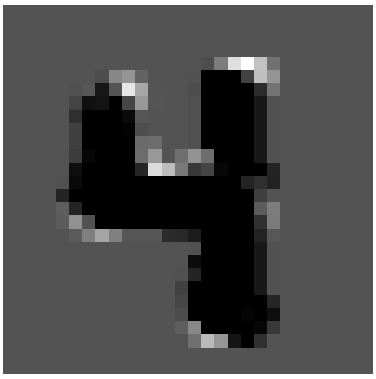
\includegraphics[width=\sideimagewidth]{ch4/assets/4_tf_feat7.png}
		\label{fig:feat7}
	}
	\\
	\subfigure[]{
		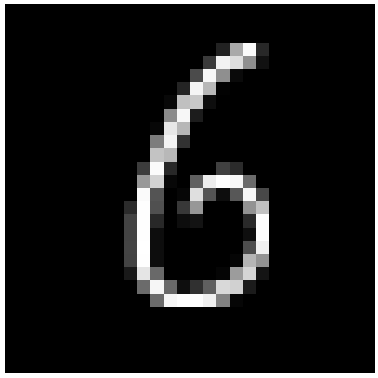
\includegraphics[width=\sideimagewidth]{ch4/assets/6_tf_original.png}
		\label{fig:6feat_ori}
	}
	\subfigure[]{
		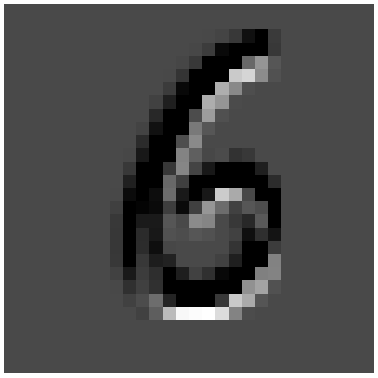
\includegraphics[width=\sideimagewidth]{ch4/assets/6_tf_feat0.png}
		\label{fig:6feat0}
	}
	\subfigure[]{
		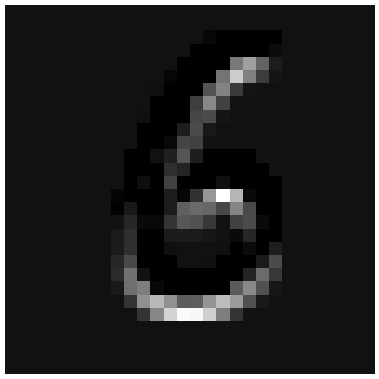
\includegraphics[width=\sideimagewidth]{ch4/assets/6_tf_feat1.png}
		\label{fig:6feat1}
	}
	\subfigure[]{
		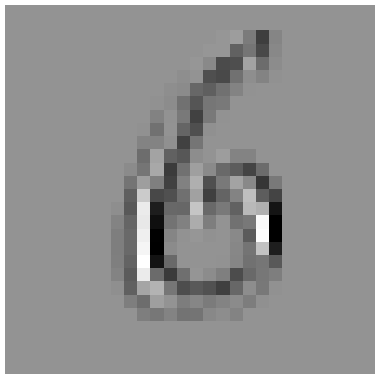
\includegraphics[width=\sideimagewidth]{ch4/assets/6_tf_feat2.png}
		\label{fig:6feat2}
	}
	\subfigure[]{
		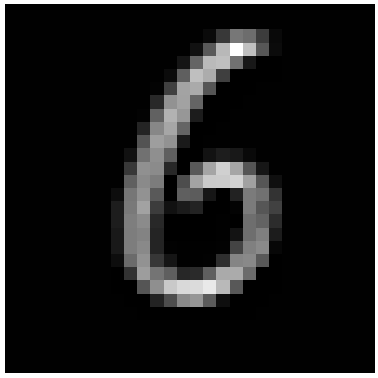
\includegraphics[width=\sideimagewidth]{ch4/assets/6_tf_feat3.png}
		\label{fig:6feat3}
	}
	\subfigure[]{
		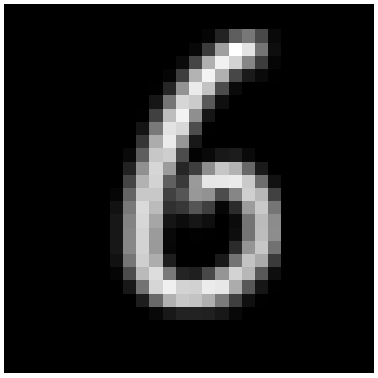
\includegraphics[width=\sideimagewidth]{ch4/assets/6_tf_feat4.png}
		\label{fig:6feat4}
	}
	\subfigure[]{
		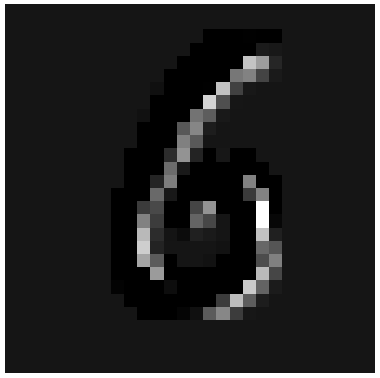
\includegraphics[width=\sideimagewidth]{ch4/assets/6_tf_feat5.png}
		\label{fig:6feat5}
	}
	\subfigure[]{
		
\includegraphics[width=\sideimagewidth]{ch4/assets/6_tf_feat6.png}
		\label{fig:6feat6}
	}
	\subfigure[]{
		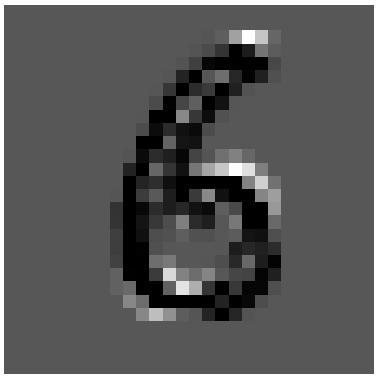
\includegraphics[width=\sideimagewidth]{ch4/assets/6_tf_feat7.png}
		\label{fig:6feat7}
	}
	\caption{Feature maps extracted from the first convolutional layer of a (real-valued) convolutional neural network with 8 filters using Tensorflow concerning the MNIST dataset. Original images are (a) and (j) for different handwritten numbers of "4" and "6" respectively.}
	\label{fig:feats}
\end{sidewaysfigure}

\begin{sidewaysfigure}
	\centering
	\begin{minipage}{\linewidth}
		\centering
		\subfigure[]{
			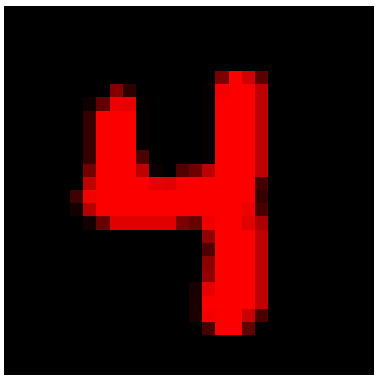
\includegraphics[width=\sideimagewidth]{ch4/assets/4_ren_ori.png}
			\label{fig:featcxy_ori}
		}
		\subfigure[]{
			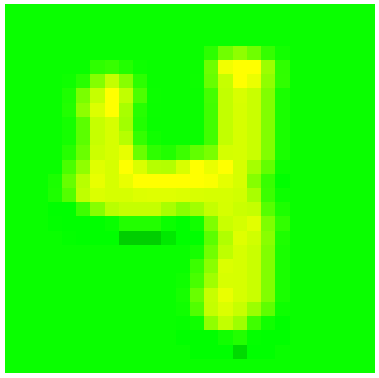
\includegraphics[width=\sideimagewidth]{ch4/assets/4xy_ren_feat0.png}
			\label{fig:featcxy0}
		}
		\subfigure[]{
			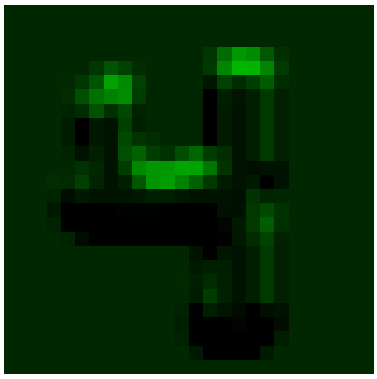
\includegraphics[width=\sideimagewidth]{ch4/assets/4xy_ren_feat1.png}
			\label{fig:featcxy1}
		}
		\subfigure[]{
			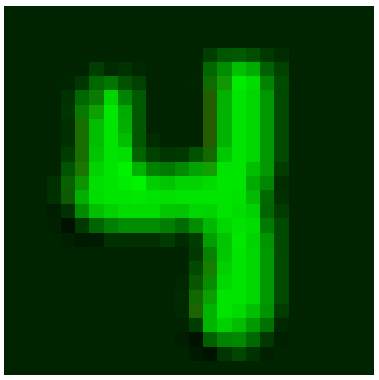
\includegraphics[width=\sideimagewidth]{ch4/assets/4xy_ren_feat2.png}
			\label{fig:featcxy2}
		}
		\subfigure[]{
			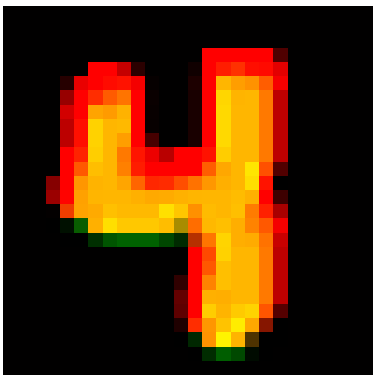
\includegraphics[width=\sideimagewidth]{ch4/assets/4xy_ren_feat3.png}
			\label{fig:featcxy3}
		}
		\subfigure[]{
			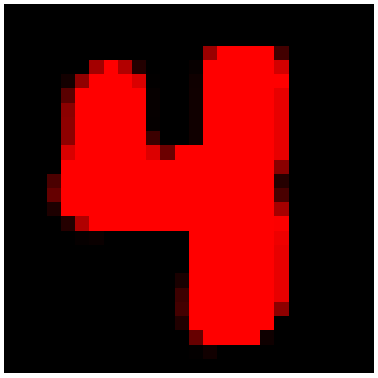
\includegraphics[width=\sideimagewidth]{ch4/assets/4xy_ren_feat4.png}
			\label{fig:featcxy4}
		}
		\subfigure[]{
			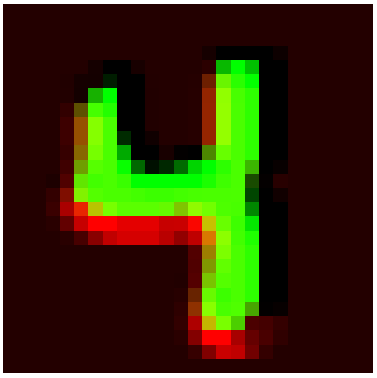
\includegraphics[width=\sideimagewidth]{ch4/assets/4xy_ren_feat5.png}
			\label{fig:featcxy5}
		}
		\subfigure[]{
			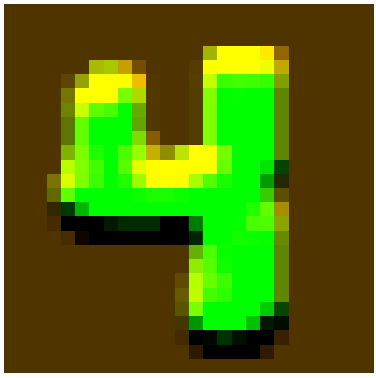
\includegraphics[width=\sideimagewidth]{ch4/assets/4xy_ren_feat6.png}
			\label{fig:featcxy6}
		}
		\subfigure[]{
			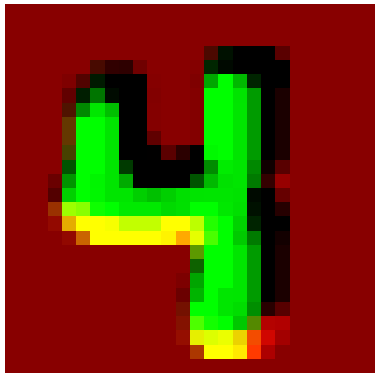
\includegraphics[width=\sideimagewidth]{ch4/assets/4xy_ren_feat7.png}
			\label{fig:featcxy7}
		}
		\\
		\subfigure[]{
			\includegraphics[width=\sideimagewidth]{ch4/assets/6_ren_ori.png}
			\label{fig:6featcxyori}
		}
		\subfigure[]{
			\includegraphics[width=\sideimagewidth]{ch4/assets/6xy_ren_feat0.png}
			\label{fig:6featcxy0}
		}
		\subfigure[]{
			\includegraphics[width=\sideimagewidth]{ch4/assets/6xy_ren_feat1.png}
			\label{fig:6featcxy1}
		}
		\subfigure[]{
			\includegraphics[width=\sideimagewidth]{ch4/assets/6xy_ren_feat2.png}
			\label{fig:6featcxy2}
		}
		\subfigure[]{
			\includegraphics[width=\sideimagewidth]{ch4/assets/6xy_ren_feat3.png}
			\label{fig:6featcxy3}
		}
		\subfigure[]{
			\includegraphics[width=\sideimagewidth]{ch4/assets/6xy_ren_feat4.png}
			\label{fig:6featcxy4}
		}
		\subfigure[]{
			\includegraphics[width=\sideimagewidth]{ch4/assets/6xy_ren_feat5.png}
			\label{fig:6featcxy5}
		}
		\subfigure[]{
			\includegraphics[width=\sideimagewidth]{ch4/assets/6xy_ren_feat6.png}
			\label{fig:6featcxy6}
		}
		\subfigure[]{
			\includegraphics[width=\sideimagewidth]{ch4/assets/6xy_ren_feat7.png}
			\label{fig:6featcxy7}
		}
		\caption{Feature maps extracted from the first convolutional layer of a complex-valued convolutional neural network with 8 filters using Tensorflow concerning the MNIST dataset. Original images are (a) and (j) for different handwritten numbers of "4" and "6" respectively. In this set, real part of the pixels is mapped in red scale and imaginary in green scale.}
		\label{fig:featscxy}
	\end{minipage}
	
	\begin{minipage}{\linewidth}
		\centering
		\subfigure[]{
			\includegraphics[width=\sideimagewidth]{ch4/assets/4_ren_ori.png}
			\label{fig:featc_ori}
		}
		\subfigure[]{
			\includegraphics[width=\sideimagewidth]{ch4/assets/4_ren_feat0.png}
			\label{fig:featc0}
		}
		\subfigure[]{
			\includegraphics[width=\sideimagewidth]{ch4/assets/4_ren_feat1.png}
			\label{fig:featc1}
		}
		\subfigure[]{
			\includegraphics[width=\sideimagewidth]{ch4/assets/4_ren_feat2.png}
			\label{fig:featc2}
		}
		\subfigure[]{
			\includegraphics[width=\sideimagewidth]{ch4/assets/4_ren_feat3.png}
			\label{fig:featc3}
		}
		\subfigure[]{
			\includegraphics[width=\sideimagewidth]{ch4/assets/4_ren_feat4.png}
			\label{fig:featc4}
		}
		\subfigure[]{
			\includegraphics[width=\sideimagewidth]{ch4/assets/4_ren_feat5.png}
			\label{fig:featc5}
		}
		\subfigure[]{
			\includegraphics[width=\sideimagewidth]{ch4/assets/4_ren_feat6.png}
			\label{fig:featc6}
		}
		\subfigure[]{
			\includegraphics[width=\sideimagewidth]{ch4/assets/4_ren_feat7.png}
			\label{fig:featc7}
		}
		\\
		\subfigure[]{
			\includegraphics[width=\sideimagewidth]{ch4/assets/6_ren_ori.png}
			\label{fig:6featc_ori}
		}
		\subfigure[]{
			\includegraphics[width=\sideimagewidth]{ch4/assets/6_ren_feat0.png}
			\label{fig:6featc0}
		}
		\subfigure[]{
			\includegraphics[width=\sideimagewidth]{ch4/assets/6_ren_feat1.png}
			\label{fig:6featc1}
		}
		\subfigure[]{
			\includegraphics[width=\sideimagewidth]{ch4/assets/6_ren_feat2.png}
			\label{fig:6featc2}
		}
		\subfigure[]{
			\includegraphics[width=\sideimagewidth]{ch4/assets/6_ren_feat3.png}
			\label{fig:6featc3}
		}
		\subfigure[]{
			\includegraphics[width=\sideimagewidth]{ch4/assets/6_ren_feat4.png}
			\label{fig:6featc4}
		}
		\subfigure[]{
			\includegraphics[width=\sideimagewidth]{ch4/assets/6_ren_feat5.png}
			\label{fig:6featc5}
		}
		\subfigure[]{
			\includegraphics[width=\sideimagewidth]{ch4/assets/6_ren_feat6.png}
			\label{fig:6featc6}
		}
		\subfigure[]{
			\includegraphics[width=\sideimagewidth]{ch4/assets/6_ren_feat7.png}
			\label{fig:6featc7}
		}
		\caption{Feature maps extracted from the first convolutional layer of a complex-valued convolutional neural network with 8 filters using Tensorflow concerning the MNIST dataset. Original images are (a) and (j) for different handwritten numbers of "4" and "6" respectively. In this set, absolute value of the pixels is mapped in red scale and phase in green scale.}
		\label{fig:featsc}
	\end{minipage}
\end{sidewaysfigure}